%======================================================================
%----------------------------------------------------------------------
%               XX                              X
%                                               X
%               XX    XXX   XXX   XXX      XXX  X  XXXX
%                X   X   X X   X X   X    X   X X X
%                X   XXXXX XXXXX XXXXX    X     X  XXX
%                X   X     X     X     XX X   X X     X
%               XXX   XXX   XXX   XXX  XX  XXX  X XXXX
%----------------------------------------------------------------------
%  	         A SKELETON FILE FOR IEEE PAPER GENERATION
%----------------------------------------------------------------------
%======================================================================

% first, uncomment the desired options:
%\documentclass[%
%        draft,
        %submission,
        %compressed,
        %final,
        %
        %technote,
        %internal,
        %submitted,
        %inpress,
        %reprint,
        %
        %titlepage,
        %notitlepage,
        %anonymous,
        %narroweqnarray,
        %inline,
        %twoside,
        %]{ieee}
%
% some standard modes are:
%
% \documentclass[draft,narroweqnarray,inline]{ieee}
% \documentclass[submission,anonymous,narroweqnarray,inline]{ieee}
 \documentclass[final,narroweqnarray,inline]{ieee}

% Use the `endfloat' package to move figures and tables to the end
% of the paper. Useful for `submission' mode.
%\usepackage {endfloat}

% Use the `times' package to use Helvetica and Times-Roman fonts
% instead of the standard Computer Modern fonts. Useful for the 
% IEEE Computer Society transactions.
% (Note: If you have the commercial package `mathtime,' it is much
% better, but the `times' package works too).
%\usepackage {times}

% In order to use the figure-defining commands in ieeefig.sty...
\usepackage{ieeefig}

% To use utf8 encoding
\usepackage[utf8]{inputenc}

\begin{document}

%----------------------------------------------------------------------
% Title Information, Abstract and Keywords
%----------------------------------------------------------------------
\title[Trabajo Practico Nº 1: Wiretapping]{%
       Trabajo Practico Nº 1: Wiretapping}

% format author this way for journal articles.
\author[SHORT NAMES]{%
	Leandro Ezequiel Barrios,
	\and
	Gonzalo Benegas,
	\and
	Martin Caravario, 
	\and
	Pedro Rodriguez 
}

% format author this way for conference proceedings
%\author[SHORT NAMES]{%
%      Martin Caravario\member{Fellow}
%      \authorinfo{%
%      Department of Electrical Engineering\\
%      Some University, Somewhere CA, 90210, USA\\
%      Phone: (xxx) xxx-xxxx, email: xxx@xxxx.xxx.xxx}
%    \and
%      Second Author\member{Senior Member}
%      \authorinfo{%
%      Department of Electrical Engineering...}
%    \and
%      and Third Author\member{Student Member}
%      \authorinfo{...}
%  }

% specifiy the journal name
%\journal{IEEE Transactions on Something, 1997}

% Or, when the paper is a preprint, try this...
%\journal{IEEE Transactions on Something, 1997, TN\#9999.}

% Or, specify the conference place and date.
%\confplacedate{Ottawa, Canada, May 19--21, 1997}

% make the title
\maketitle               

% do the abstract

\begin{abstract}
En el presente Trabajo Práctico utilizaremos algunas de las técnicas
provistas por la teoría de la información para estudiar y analizar algunas
redes de información. El objetivo será distinguir diversos aspectos de la
red de manera analítica. Para cumplir con nuestro objetivo, haremos uso de
dos herramientas modernas de manipulación y análisis de paquetes: Wireshark
y Scapy.
\end{abstract}

% do the keywords
%\begin{keywords}
%keyword 1, keyword 2 ...
%\end{keywords}

% start the main text ...
%----------------------------------------------------------------------
% SECTION I: Introduction
%----------------------------------------------------------------------
\section{Primera consigna}

\subsection{}
Para realizar esta consigna construimos un script en python que hace uso de la
función ``sniff'', provista por Scapy. Este nos permitió escuchar durante
cierto tiempo la red local y guardarnos todos los paquetes que llegaban a
nuestra placa de red y eran levantados por esta. A partir de estos datos
que guardamos, seremos capaces de encontrar  nodos y protocolos
distinguidos en la red a partir de gráficos de torta e histogramas.

\subsection{}
ARP es un protocolo de la capa de enlace de datos, responsable de encontrar
la dirección de capa 2 (Ethernet MAC) que corresponde a una determinada
dirección IP (dirección de capa 3 de enlace). Es decir, cada vez que un host
quiere comunicarse con otro y su dirección MAC no se encuentra dentro de su
tabla ARP, debe enviar un paquete who-has broadcast para determinar la dirección MAC
del host destino. De este modo, todos los hosts del dominio de colisión de
esta máquina reciben dicho paquete, siendo respondido el mismo únicamente
por el host requerido, mediante un paquete rep, mediante un paquete reply.
Para distinguir nodos (símbolos) en este contexto, tomamos a aquellos cuya
probabilidad de aparición era alta, de forma tal que la información provista
por el mismo sea menor a la entropía de la fuente a la cuál el símbolo
pertenece.

\medskip
Para este ejercicio se decidi\'o tomar la siguiente fuente: \\ 
$S_{1}$ = \{$s_{1} \dots s_{n}$\} siendo el símbolo $s_{i}$ la tupla (src, dst), donde
src y dst son respectivamente las direcciones ip del emisor y receptor del
paquete ARP escuchado.  \\
Al analizar esta fuente, se busca identificar los nodos distinguidos. Es
decir, aquellos pares de ip que podemos concluir tienen mayor probabilidad de comunicarse
entre sí en la red escuchada, a partir de los datos obtenidos. 


\section{Experimentacion}


\subsection{Experimento 1}
Para este experimento se analiz\'o el trafico dentro de la red LAN de la empresa Techint, escuchando pasivamente
en la red durante media hora, con la herramienta desarrollada en el ejercicio 1. \\
Los resultados del experimento seran divididos segun la fuente utilizada (S o $S_{1}$), para poder analizar
entropias e informacion de sus respectivos simbolos de forma adecuada. \\
Los resultados obtenidos fueron los siguientes: 

\subsubsection{Fuente utilizada: S}

% \begin{figure}
% \begin{center}
%   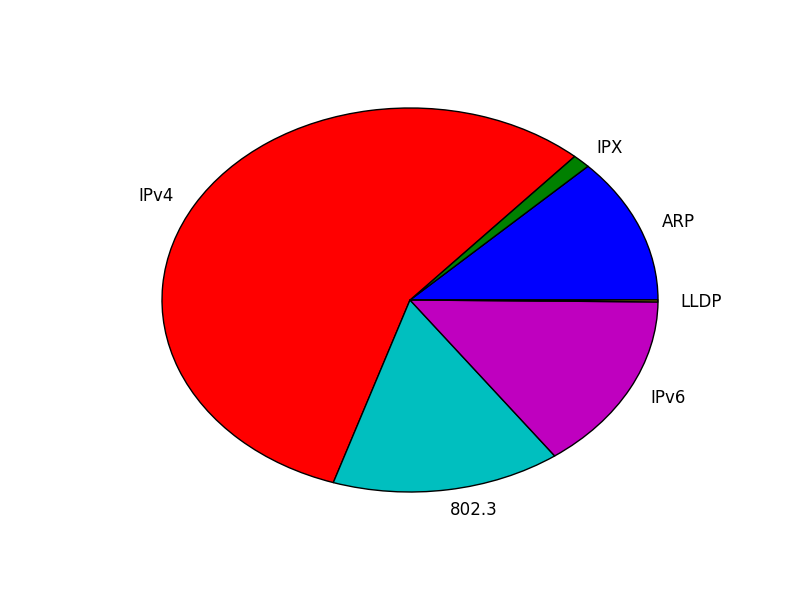
\includegraphics[width=0.5\textwidth]{graficos/techint-pie.png}
%   \caption{Techint - Gráfico torta}
%   \label{techint-pie}
% \end{center}
% \end{figure}

%\begin{figure}
%\begin{center}
%  \includegraphics[width=0.5\textwidth]{../output/labosdc-20150428-pie.png}
%  \caption{Labosdc20150428 - pie}
%  \label{labosdc20150428-pie}
%\end{center}
%\end{figure}

%{Grafico que muestra la proporción de cada protocolo dentro del total}
En este gráfico de torta se observa la cantidad de paquetes escuchados de cada
protocolo. Se pudieron escuchar protocolos de tipo IPv4, IPX, ARP, LLDP,
802.3 e IPv6. El símbolo mayormente emitido (con mayor probabilidad de
aparecer) por la fuente es IPv4.

\begin{figure}
\begin{center}
  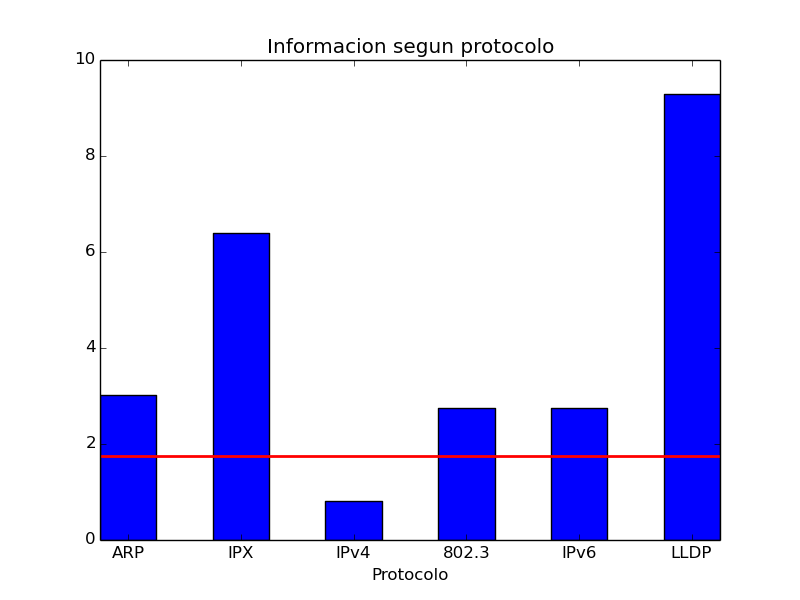
\includegraphics[width=0.5\textwidth]{graficos/techint_histogram.png}
  \caption{Techint - Histograma}
  \label{techint-pie}
\end{center}
\end{figure}

%{Grafico que muestra la información que aporta cada protocolo y el corte de
%la entropía}
Este histograma muestra la cantidad de información provista por cada símbolo
de la fuente $S$ definida, calculada según la fórmula $ I(s_{i}) =
-log(p(s_{i}))  $. También hay un corte en la entropía de la fuente
(aproximadamente 1,9), que nos permite observar de manera sencilla cómo el símbolo (nodo)
distinguido de la fuente es IPv4.

\subsubsection{Fuente utilizada: $S_{1}$}


% try out a theorem...
%\newtheorem{theorem}{Theorem}

%\begin{theorem}[Theorem name]
%  Consider the system ...
%\end{theorem}

%\begin{proof}
%  The proof is trivial.
%\end{proof}

% do the biliography:
\bibliographystyle{IEEEbib}
\bibliography{my-bibliography-file}

% where ``my-bibliography-file.bib'' is the name of the file with all the 
% BibTeX entries.

% do the biographies...
%\begin{biography}{Gregory L. Plett}
%  A bio with no face...
%\end{biography}

% If you want a picture with your biography, then specify the name of
% the postscript file in square brackets. That is, uncomment the
% following three lines and change the name of "face.ps" to the name of 
% your file.
%\begin{biography}[face.ps]{Gregory L. Plett}
%  A bio with a face...
%\end{biography}

%----------------------------------------------------------------------
% FIGURES
%----------------------------------------------------------------------
% There are many ways to include figures in the text. We will assume
% that the figure is some sort of EPS file.
%
% The outdated packages epsfig and psfig allow you to insert figures
% like: \psfig{filename.eps} These should really be done now using the
% \includegraphics{filename.eps} command.  
%
% i.e.,
%
% \includegraphics{file.eps}
%
% whenever you want to include the EPS file 'file.eps'. There are many
% options for the includegraphics command, and are outlined in the
% on-line documentation for the "graphics bundle". Using the options,
% you can specify the height, total height (height+depth), width, scale,
% angle, origin, bounding box "bb",view port, and can trim from around
% the sides of the figure. You can also force LaTeX to clip the EPS file
% to the bounding box in the file. I find that I often use the scale,
% trim and clip commands.
% 
% \includegraphics[scale=0.6,trim=0 0 0 0,clip=]{file.eps}
% 
% which magnifies the graphics by 0.6 (If I create a graphics for an
% overhead projector transparency, I find that a magnification of 0.6
% makes it look much better in a paper), trims 0 points off
% of the left, bottom, right and top, and clips the graphics. If the
% trim numbers are negative, space is added around the figure. This can
% be useful to help center the graphics, if the EPS file bounding box is
% not quite right.
% 
% To center the graphics,
% 
% \begin{center}
% \includegraphics...
% \end{center}
% 
% I have not yet written good documentation for this, but another 
% package which helps in figure management is the package ieeefig.sty,
% available at: http://www-isl.stanford.edu/people/glp/ieee.shtml
% Specify:
% 
%\usepackage{ieeefig} 
% 
% in the preamble, and whenever you want a figure,
% 
%\figdef{filename}
% 
% where, filename.tex is a LaTeX file which defines what the figure is.
% It may be as simple as
% 
% \inserteps{filename.eps}
%
% or
% \inserteps[includegraphics options]{filename.eps}
% 
% or may be a very complicated LaTeX file. 

\end{document}
